\documentclass[10pt]{article}
\usepackage[margin=0.75in]{geometry}
\usepackage{graphicx}
\usepackage{booktabs}
\usepackage{tikz}
\usetikzlibrary{positioning,arrows.meta,fit}
\usepackage{enumitem}
\usepackage{amsmath}
\usepackage{caption}
\usepackage[compact]{titlesec}
\usepackage[hidelinks]{hyperref}
\usepackage{needspace}
\setlist{nosep,leftmargin=*}
\setlength{\parskip}{4pt}
\setlength{\parindent}{0pt}
\setlength{\emergencystretch}{1em}
\clubpenalty=10000
\widowpenalty=10000

% shows the screenshot if the file exists, otherwise a box saying what goes there
\newcommand{\screenshot}[4][3.2in]{%
  \IfFileExists{images/#2}{\includegraphics[width=#3,height=#1,keepaspectratio]{images/#2}}{%
    \fbox{\parbox[c][1.2in][c]{#3}{\centering\small Screenshot goes here: \texttt{\detokenize{images/#2}}\\ (#4)}}}}

\begin{document}
\begin{center}
{\Large\bfseries CS6650 Assignment 2: Message Queue, Consumers and the Real Leaderboard}\\[4pt]
Nikhil Pawar \quad | \quad November 2026
\end{center}

\section{Git Repository}
\url{https://github.com/aimsotrash/cs6650-assignments}, folder \texttt{assignment-2/}:\\
\texttt{/server-v2}, \texttt{/consumer}, \texttt{/deployment}, \texttt{/monitoring}, \texttt{/results}, \texttt{AI\_USAGE.md}. The load client is my Assignment 1 client (\texttt{assignment-1/client-part2}), unchanged.

% ======================= ARCHITECTURE DOCUMENT (2 pages max) =======================
\section{Architecture Document}

\subsection{System Architecture}
Every host is an m8azn.large (2 cores at 5.0 GHz; the Learner Lab allows sizes up to \texttt{.large}, and this is the fastest one) in us-west-2a, set up as in Lab 1 (Amazon Linux 2023, Corretto 11, Tomcat 9). The ingest server is my Assignment 1 WAR with two changes: a valid swipe is published to RabbitMQ instead of just returning 201, and the WebSocket endpoint pushes real leaderboards that arrive over a backplane instead of a fake one. A separate consumer app does the aggregation. RabbitMQ 4.4 runs on its own instance, installed from rabbitmq.com's RPM repository.

\begin{center}
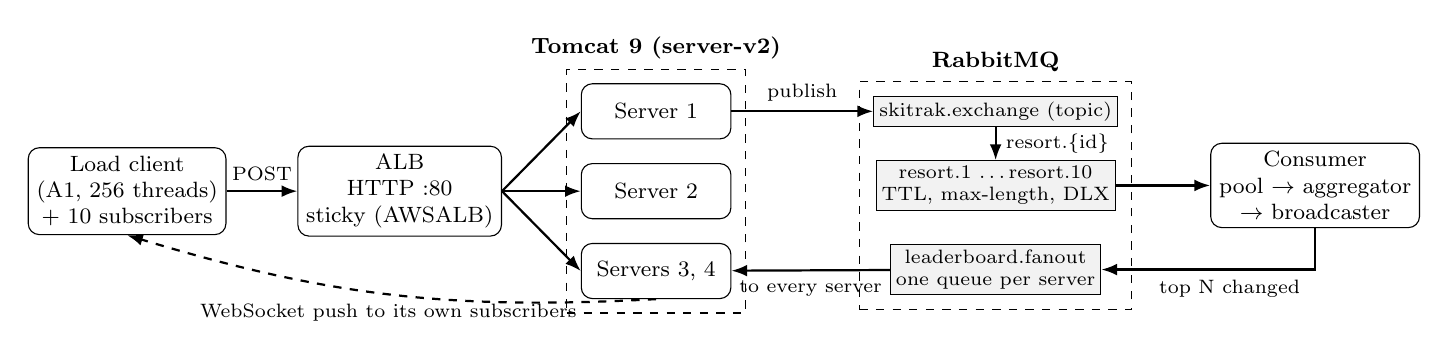
\begin{tikzpicture}[
  box/.style={draw, rounded corners, align=center, font=\footnotesize, inner sep=3pt, minimum height=0.7cm},
  q/.style={draw, align=center, font=\scriptsize, inner sep=2pt, fill=black!5},
  arrow/.style={-{Latex[length=2mm]}, thick}]
  \node[box] (client) {Load client\\(A1, 256 threads)\\+ 10 subscribers};
  \node[box, right=0.9cm of client] (alb) {ALB\\HTTP :80\\sticky (AWSALB)};
  \node[box, right=1.0cm of alb, minimum width=1.9cm] (s2) {Server 2};
  \node[box, above=0.3cm of s2, minimum width=1.9cm] (s1) {Server 1};
  \node[box, below=0.3cm of s2, minimum width=1.9cm] (s3) {Servers 3, 4};
  \node[q, right=1.8cm of s1] (ex) {skitrak.exchange (topic)};
  \node[q, below=0.42cm of ex] (rq) {resort.1 \dots resort.10\\TTL, max-length, DLX};
  \node[q, below=0.42cm of rq] (fan) {leaderboard.fanout\\one queue per server};
  \node[box, right=1.2cm of rq] (cons) {Consumer\\pool $\to$ aggregator\\$\to$ broadcaster};
  \node[draw, dashed, fit=(ex)(rq)(fan), inner sep=5pt, label={[font=\footnotesize\bfseries]above:RabbitMQ}] {};
  \node[draw, dashed, fit=(s1)(s2)(s3), inner sep=5pt, label={[font=\footnotesize\bfseries]above:Tomcat 9 (server-v2)}] {};
  \draw[arrow] (client) -- node[above, font=\scriptsize]{POST} (alb);
  \draw[arrow] (alb) -- (s2);
  \draw[arrow] (alb.east) -- (s1.west);
  \draw[arrow] (alb.east) -- (s3.west);
  \draw[arrow] (s1) -- node[above, font=\scriptsize]{publish} (ex);
  \draw[arrow] (ex) -- node[right, font=\scriptsize]{resort.\{id\}} (rq);
  \draw[arrow] (rq) -- (cons);
  \draw[arrow] (cons) |- node[pos=0.7, below, font=\scriptsize]{top N changed} (fan);
  \draw[arrow] (fan) -- node[below, font=\scriptsize]{to every server} (s3);
  \draw[arrow, dashed] (s3.south) to[bend left=10] node[below, font=\scriptsize]{WebSocket push to its own subscribers} (client.south);
\end{tikzpicture}
\captionof{figure}{Architecture. Swipes go Client $\to$ ALB $\to$ any server $\to$ queue $\to$ consumer; leaderboards come back through the fanout to every server, which pushes them to the subscribers it holds.}
\end{center}

\subsection{Swipe to Leaderboard (sequence)}
\begin{center}
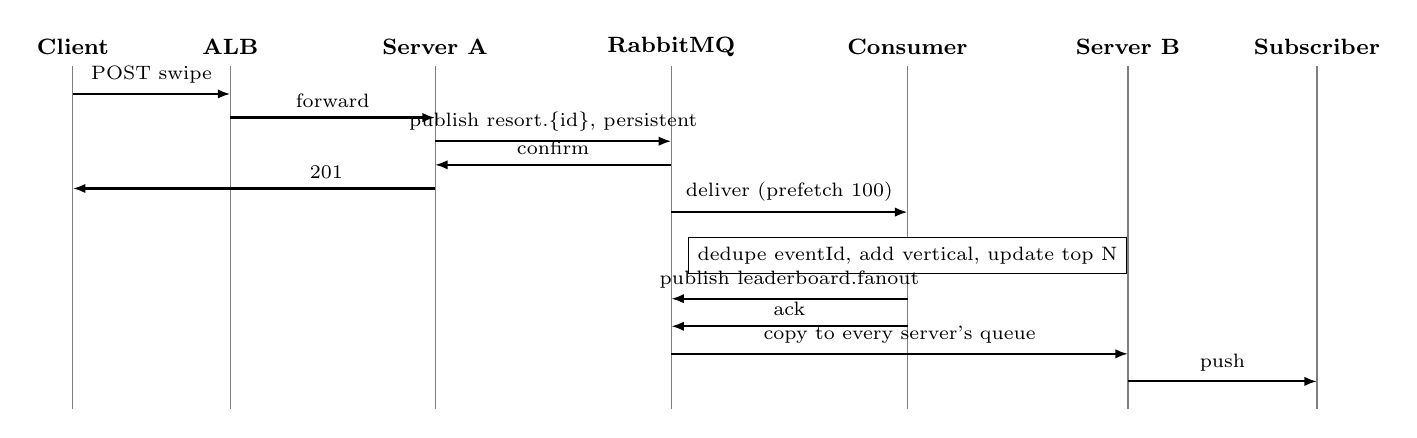
\begin{tikzpicture}[font=\scriptsize, arrow/.style={-{Latex[length=1.6mm]}, thick}]
  \foreach \x/\n in {0/Client, 2.0/ALB, 4.6/Server A, 7.6/RabbitMQ, 10.6/Consumer, 13.4/Server B, 15.8/Subscriber} {
    \node[font=\footnotesize\bfseries] at (\x, 0) {\n};
    \draw[gray] (\x, -0.25) -- (\x, -4.6);
  }
  \draw[arrow] (0,-0.6) -- node[above]{POST swipe} (2.0,-0.6);
  \draw[arrow] (2.0,-0.9) -- node[above]{forward} (4.6,-0.9);
  \draw[arrow] (4.6,-1.2) -- node[above]{publish resort.\{id\}, persistent} (7.6,-1.2);
  \draw[arrow] (7.6,-1.5) -- node[above]{confirm} (4.6,-1.5);
  \draw[arrow] (4.6,-1.8) -- node[above, pos=0.3]{201} (0,-1.8);
  \draw[arrow] (7.6,-2.1) -- node[above]{deliver (prefetch 100)} (10.6,-2.1);
  \node[draw, fill=white, align=center] at (10.6,-2.65) {dedupe eventId, add vertical, update top N};
  \draw[arrow] (10.6,-3.2) -- node[above]{publish leaderboard.fanout} (7.6,-3.2);
  \draw[arrow] (10.6,-3.55) -- node[above]{ack} (7.6,-3.55);
  \draw[arrow] (7.6,-3.9) -- node[above]{copy to every server's queue} (13.4,-3.9);
  \draw[arrow] (13.4,-4.25) -- node[above]{push} (15.8,-4.25);
\end{tikzpicture}
\captionof{figure}{One swipe. The 201 means the broker has the message; the leaderboard is updated asynchronously. Server A and Server B are usually different servers.}
\end{center}

\subsection{Queue Topology}
\begin{itemize}
  \item \texttt{skitrak.exchange} (topic, durable), routing key \texttt{resort.\{resortID\}}, bound to one durable queue per resort, \texttt{resort.1} to \texttt{resort.10}. Each queue has a 1 h message TTL, a 200,000 message limit with \texttt{x-overflow: reject-publish} (a full queue nacks the publish, the server answers 503 and the client retries; the default would silently drop the oldest swipe), and dead-letter exchange \texttt{skitrak.dlx} $\to$ \texttt{skitrak.dead} for poison and expired messages.
  \item \texttt{leaderboard.fanout} (fanout): every ingest server binds its own broker-named, exclusive, auto-delete queue (newest 1,000 messages). The consumer publishes with routing key \texttt{resort.\{id\}}, which the fanout ignores but passes along, so a server knows the resort without parsing.
  \item The server and the consumer both declare all of this on connect, so start order doesn't matter.
\end{itemize}

\subsection{Connection Locality: Broadcast Backplane}
A WebSocket connection lives on the server that accepted it, but the consumer that computes the new standings runs on another host. I chose a \textbf{broadcast backplane}: the consumer publishes each changed leaderboard (the whole top N for that resort and day) to \texttt{leaderboard.fanout}, every server gets a copy, and each one pushes it to the sessions it holds for that resort. Why: any server can hold any subscriber, so the ALB can spread connections freely and stickiness only matters for reconnects; adding a server just adds one more bound queue; the consumer doesn't need to know where subscribers are; and the broker I already run is the pub/sub layer (Week 6). The cost is that every server receives every update, even for resorts it has no subscribers for, and there is one extra broker hop. That is small here: about 2,900 updates per 500,000 swipes (0.6\% of the messages). \textbf{Co-location} (route a resort's swipes and its WebSocket connections to the same node) would need resort-aware routing in the ALB and the aggregation inside the ingest servers; a busy resort couldn't be spread, a failed node would take its resorts with it, and it can't scale past the 10 resorts.

\subsection{Threading Model}
\begin{itemize}
  \item \textbf{Server:} Tomcat's request threads publish through a \texttt{ChannelPool}: one connection and 64 channels in confirm mode. A thread borrows a channel, publishes, waits for the confirm (5 s timeout) and returns it, so a channel is never used by two threads and there is no channel per publish. The backplane listener is one consumer thread on its own connection; it sends to each session in blocking mode with a 1 s timeout, so a stalled client can't hold up the others for long.
  \item \textbf{Consumer:} \texttt{CONSUMER\_THREADS} channels, each with a thread, and the 10 resort queues given out round robin (fair distribution). A resort's queue is consumed by exactly one channel, and the RabbitMQ client hands a channel's messages to one thread at a time in order, so each resort's swipes are applied in order; that also caps useful threads at 10. Dynamic scaling: every 5 s, if more than 1,000 swipes are waiting the pool doubles its threads (up to \texttt{MAX\_THREADS}); after 30 s under 100 it halves them. A rescale cancels every consumer, waits for cancel-ok (sent after the delivered messages are done), acks what's left and restarts, so order holds across it.
  \item \textbf{State and acks:} \texttt{ConcurrentHashMap}s \texttt{skierVertical} (resort:day:skier), \texttt{resortLeaderboards} (resort:day $\to$ synchronized \texttt{TopN}, N = 20) and an \texttt{AtomicLong} counter. Prefetch 100; one ack per 50 messages (\texttt{multiple = true}), with the rest of a batch acked by a flush every 5 s. Broadcasts go through one lock on one channel of a separate connection, so a broker that blocks publishers doesn't stop the acks.
\end{itemize}

\subsection{Load Balancing}
Internet-facing ALB, HTTP :80 to the servers on :8080; target group health check \texttt{GET /skitrak/health} every 30 s, timeout 5 s, healthy 2, unhealthy 3; sticky sessions with the ALB cookie (\texttt{AWSALB}, 1 day); idle timeout 120 s; WebSocket needs no switch on an ALB. Its security group allows the client's public IP (the ALB's name resolves to public IPs even inside the VPC). A new ALB starts with small nodes, so I warm it up with about 5 minutes of steady load before measuring (Section~3).

\subsection{Failure Handling}
\begin{itemize}
  \item \textbf{Dropped connection:} the pool notices a closed connection on the next borrow and reconnects (at most one attempt a second, so while the broker is down requests fail fast with 503). Heartbeat 10 s, so a vanished broker is noticed quickly. The consumer and the backplane listener use the client library's automatic recovery.
  \item \textbf{No loss, no double count:} manual ack after aggregation (at least once); dedupe on \texttt{eventId} (the last 50,000 per resort); 201 only after the publisher confirm; if a publish fails, one retry with the same \texttt{eventId}, so a copy that did get in is dropped by the dedupe.
  \item \textbf{Poison messages:} unreadable $\to$ rejected to the dead-letter queue; failed processing $\to$ requeued once, then dead-lettered (Week 6).
  \item \textbf{Consumer:} systemd \texttt{Restart=always}, health check \texttt{:8081/health}, graceful shutdown (cancel, finish, ack, close). State is in memory, so a crash loses the totals (persistence is Assignment 3).
\end{itemize}

\label{end-of-design}
% ======================= TEST RESULTS =======================
\clearpage
\section{Test Results (every host m8azn.large)}
Final settings: the Assignment 1 client unchanged with 256 threads; 64 channels per server; consumer with 10 threads, prefetch 100, one ack per 50 messages, ZGC; \texttt{TOP\_N} 20; ALB warmed up first. Throughput is swipes that got a 201 per second (overall, and in the main phase after the client's 32-thread warmup). Every run: \textbf{0 failed swipes} and the consumer applied exactly as many swipes as the client sent (no loss, no double count); with one client, the leaderboard updates its 10 subscribers received equal the broadcasts the consumer published.
\begin{center}
\footnotesize
\setlength{\tabcolsep}{4pt}
\resizebox{\textwidth}{!}{\begin{tabular}{lrrrr}
\toprule
\textbf{One client host} & \textbf{1 server (no ALB)} & \textbf{ALB + 2 servers} & \textbf{ALB + 4 servers} & \textbf{ALB + 4 servers} \\
\midrule
Swipes & 500,000 & 500,000 & 500,000 & 1,000,000 \\
Throughput overall (main phase) & 33,602/s (36,217) & 34,758/s (40,068) & 34,199/s (39,284) & \textbf{42,032/s} (45,019) \\
Ingest latency mean / p99 & 6.6 / 25.7 ms & 6.1 / 13.9 ms & 6.2 / 14.6 ms & 5.5 / 12.7 ms \\
Queue depth peak / average & 263 / 158 & 336 / 215 & 367 / 168 & 385 / 223 \\
Consumer lag (accept $\to$ applied) avg / max & 2 / 95 ms & 1 / 26 ms & 0 / 60 ms & 1 / 66 ms \\
Leaderboard updates received = broadcasts & 2,785 & 2,894 & 2,909 & 3,716 \\
Push latency (consumer $\to$ subscriber) mean / p99 & 1.0 / 9 ms & 1.7 / 16 ms & 1.7 / 10 ms & 1.4 / 13 ms \\
Swipes per server & 500,000 & 249,998--250,002 & 124,999--125,002 & 249,999--250,002 \\
CPU: broker / each server / client / consumer & 75 / 50 / 81 / 16\% & 90 / 31--38 / 95 / 23\% & 81 / 12--16 / 86 / 16\% & 97 / 18--20 / 91 / 23\% \\
\midrule
\textbf{Two client hosts} (same client on both) & 500K + 500K & 500K + 500K & 500K + 500K & 1M + 1M \\
\midrule
Throughput overall (main phase), sum & 40,185/s (41,755) & 44,618/s (47,733) & 45,046/s (48,459) & \textbf{46,887/s} (49,001) \\
Ingest latency mean / queue peak / lag max & 11.5 ms / 319 / 117 ms & 10.0 ms / 380 / 145 ms & 10.0 ms / 430 / 150 ms & 10.1 ms / 433 / 184 ms \\
CPU: broker / each server & 98 / 60\% & -- & 98 / 20--26\% & 100 / 22--25\% \\
\bottomrule
\end{tabular}}
\end{center}
The 1M one-client run is the one with the client's JVM on the parallel garbage collector (\texttt{java -XX:+UseParallelGC -jar}, same jar); with the default G1 it gave 39,430/s (42,032 main phase), and a rerun with the parallel GC gave 41,846/s. The first two-client ALB + 2 run gave 44,366/s with one 5-second queue sample at 1,544 (all other samples 213--359); the rerun is in the table.

\textbf{Warming up the ALB.} My first runs on every new ALB were stuck at about 11.5K swipes/s per client at 20 ms with every host mostly idle (ALB + 4: 11,550/s); at first I took that as the cost of the ALB hop. A new ALB starts with small nodes: under steady load (2 clients $\times$ 4M swipes) it added nodes after 3--5 minutes and its DNS name moved to them. The Java client looks the name up once and keeps its connections, so only runs started after that use the new nodes. Same servers and client afterwards: 34,199/s instead of 11,550/s.

\textbf{Performance analysis.} With one client host, the client (81--95\% CPU) and the broker (75--97\%) both run out near 40K/s, so 1, 2 and 4 servers are close (33.6K $\to$ 34.8K $\to$ 34.2K overall, 36.2K $\to$ 40.1K $\to$ 39.3K main phase) and the ALB runs have lower tail latency (p99 14 vs 26 ms). To find the next bottleneck I ran the same client on two hosts at once: one server tops out at 40.2K/s (its requests queue for Tomcat's 200 threads and its single AMQP connection, at 60\% CPU), while 2 and 4 servers reach 44.6K and 45.0K/s (+11--12\%, main phase +14--16\%). After that the single broker (98--100\% of its 2 cores) is the limit, so 2 $\to$ 4 servers adds little; the highest throughput was \textbf{46,887/s} (49,001 main phase) with 2M swipes through ALB + 4. Consumer lag averaged 0--5 ms in every run, but its maximum went over 100 ms (117--184 ms) in the two-client runs, where the broker was saturated; up to 42K/s it stayed under 100 ms.

\textbf{How I got there} (1M through the ALB, one change at a time): 128 client threads 25,450/s; 256 threads 26,647/s; one ack per 50 messages 27,762/s (less broker CPU); consumer on ZGC 28,134/s; warmed-up ALB 39,430/s; client JVM on the parallel GC 42,032/s. No gain: 384 or 512 client threads (36.5K, 34.1K/s: Tomcat runs 200 requests at once and the 2-core client spends the rest on threads), one ack per 100 with prefetch 250 (39.9K/s, deeper queue), turning off the broker's Erlang scheduler busy-waiting (39.4K/s). \textbf{The GC change fixed the queue profile:} with G1, one 5 s sample per run jumped over 1,000 because at 30K swipes/s a 40 ms consumer GC pause queues about 1,200 swipes; with ZGC every run stayed at 140--430 (Figure~\ref{fig:fast}).

\begin{center}
\screenshot[2.9in]{rabbitmq_overview_fast.png}{\textwidth}{RabbitMQ overview during a 1M run}
\captionof{figure}{RabbitMQ, 1M through the ALB with the final consumer settings (before the ALB warm-up, last minute): publish, confirm, deliver and ack on one flat plateau at about 30K/s; 140--330 messages queued during the run (stable, no sawtooth), 0 ready and 0 unacked right after it.}
\label{fig:fast}
\end{center}

\begin{center}
\screenshot[2.2in]{alb_warm.png}{\textwidth}{ALB CloudWatch metrics for the final runs}
\captionof{figure}{ALB (CloudWatch, UTC) for the final runs: the new ALB from 05:53, the warm-up load 06:00--06:05 (one ELB 5XX while it added nodes; the client retried it), then the measured runs, each 1M run peaking in its busiest minute; requests per target are half or a quarter of the total (2 or 4 healthy targets).}
\end{center}

\textbf{Sticky sessions:} with probes counted in each server's Tomcat access log (\texttt{results/stickiness/}), the ALB split 8 cookieless requests 4/4, while with the \texttt{AWSALB} cookie 8/8 HTTP requests and 5/5 WebSocket upgrades went to the same server. \textbf{Dropped connections:} force-closing every AMQP connection mid-run (40K swipes) gave 0 failed, 0 retries; the server logged \texttt{reconnected to rabbit, 64 channels}, the consumer and backplane recovered, and the dedupe dropped 13 duplicate copies (applied = sent). \textbf{Real leaderboards:} besides updates received = broadcasts in every one-client run, the resort 3 WebSocket through the ALB got 17 updates in 8 s during a 1M run (\texttt{websocket\_sample.txt}): the top 20 changes as swipes arrive, with verticals summed from \texttt{lift\_vertical.json}.

\end{document}
